\documentclass{article}
\usepackage{url}
\usepackage{amsmath}
\usepackage{booktabs}
\usepackage{longtable}
\usepackage{tikz}
\usepackage{listings}
\usetikzlibrary{positioning}
\newcommand{\colAwidth}{0.2\textwidth}
\newcommand{\colBwidth}{0.7\textwidth}
\begin{document}

\bibliographystyle{plain}
\pagestyle{plain}
\thispagestyle{empty}
\markboth{{\sc thesis proposal}}{{\sc thesis proposal}}
\def\title{\large \sc Literate Software and the Drasil Framework}
\def\author{\sc Dan Szymczak}
\def\studnum{0759661}
\def\email{\sc szymczdm@mcmaster.ca}

\def\degree{Doctor of Philosophy}
\def\deptname{Computing and Software}
\def\supJ{Jacques Carette}
\def\supS{Spencer Smith}

\def\submissiondate{\today}
\def\completiondate{August 2018}

\begin{center}
{\Large \bf 
   McMaster University
\\ Department of \deptname \\}
\vspace{.25in}
{\Large \bf
   Proposal for Thesis Research in Partial Fulfillment
 of the Requirements for the Degree of \degree \\}
\end{center}

\vspace{.5in}

\begin{tabular}{rlc}
   {\large \sc Title:}                       & \multicolumn{2}{l}{\title}
\\ {\sc Submitted by:}
                            & \author  & \\
    {\sc Student Number:}   & \studnum & \\
                            & \email   & \\ 
			    &	       &
\\ { \sc Date of Submission:}          & \multicolumn{2}{l}{\submissiondate}
\\ {\small \sc Expected Date of Completion:} & \multicolumn{2}{l}{\completiondate}
\\ & \\ & \\
\\ {\large \sc Supervisors:}                 & {\large {\supJ}}
\\ & {\large {\supS}}
\end{tabular}

\cleardoublepage
\pagenumbering{roman}
\begin{abstract}

The current state of Scientific Computing software development leaves room for
improvement. There is a need for improved software quality, more consistent use
of software engineering practices, and reduced information duplication. As it
stands, information duplication creates a number of problems. Traceability is
hard to achieve as finding the source of a
piece of information is difficult among the possibilities. Over time
this impacts the maintainability of a piece of software, as developers may not
be able to track down the source of a problem. Also, with many duplicated
information sources, it makes creating documentation more tedious, reducing a
developer's desire to produce and maintain high-quality documentation. I want to
facilitate the improvement of qualities (maintainability, traceability,
reproducibility, etc.) across all artifacts of a piece of software. I believe a
knowledge-based approach, which borrows ideas from literate programming, and
involves a larger short-term investment from developers is the first step to
improving software as a whole. I am creating a framework (Drasil) to facilitate
this approach, focusing on avoiding knowledge duplication, while improving
traceability and automating as much of the development process as possible.
I believe with the proper tools for automation we can ensure good software
engineering practices are followed (regardless of the developer's background)
and improve the overall quality of software.

\end{abstract}
\pagebreak
\tableofcontents
\pagebreak
\pagenumbering{arabic}

\section{Introduction}

%I want everyone to make better software. I believe this can be achieved by
%improving software qualities such as maintainability, traceability,
%verifiability, reproducibility, and reusability. As that is too broad of a
%target, I will be focusing on well-understood domains; specifically Scientific
%Computing (SC). SC has a very rich, well-understood background, but tends to
%suffer from a lack of high-quality software and tools. In many cases, SC
%developers are scientists first and lack a strong software engineering
%background.

Scientists and engineers rely heavily on models that share common
mathematical/scientific knowledge. These are shared, in textbook form, across
many projects. However, when it comes to implementing software, this information
is then duplicated for each project, as well as being duplicated within the
project (in requirements, design documents, code and tests, for example). It
should be possible to capture this knowledge once, and then re-use it, first
within the same project but in different views (documents/contexts), then across
many projects. I want to create a system that deals with this issue of
information duplication, especially for the knowledge contained in scientific
models.

As it stands, information duplication can have a direct impact on qualities such
as maintainability, traceability, verifiability, and reproducibility. Consider a
project containing (at least) these four software artifacts: Software Requirements
Specification (SRS), design document, source code, and a testing document. As
the project evolves, some of the knowledge contained within it will inevitably
change due to changing requirements, new design decisions, technical or resource
limitations, etc. Updating the software artifacts to reflect these changes is
tedious; a developer must trace their way through each of the artifacts to
ensure new information has been added (new requirements and/or design
decisions), the change does not cause conflicts,
%with existing requirements/design/assumptions/test cases 
and any assumptions made or test cases to be used are still applicable (or are
appropriately removed/updated).

Now consider a software project with more artifacts: each change to the
knowledge becomes even more tedious to propagate.
%Can I say the following?
It is not uncommon for developers to lack the resources or motivation to update
each artifact to accommodate every minor change.

As artifacts in a software project begin to fall out of sync with each other,
the qualities of the project as a whole suffer. Consider traceability: if the
artifacts in a software project are inconsistent with each other, how can one
accurately analyze a change or validate a requirement? On a similar note, how
easy is it to maintain a system if one cannot track where a problem came from?

%TODO: I intend to ... Show that this is an opportunity for improvement.


%
%Multiple implementations of the same model is not my only concern involving
%duplication. A typical software project involves many different software
%artifacts (requirements and design documents, test cases, source code, manuals,
%etc.), each of which contain (some subset of) the same underlying scientific
%knowledge. Essentially, this knowledge is duplicated as necessary into each of
%the requisite artifacts for a project. As the project evolves, some of this
%knowledge will inevitably change, leading to issues with inter-artifact
%consistency until someone manually updates each artifact after the change is
%made. With small changes, these updates can be done fairly quickly (though it
%may be tedious), but for larger changes the update process for each artifact is
%far more resource intensive. Oftentimes, these changes are not recorded across all artifacts due to a lack of resources.

%I intend to find a way to handle the massive amount
%of inter-artifact knowledge duplication using a resource-friendly means. 
%%Again, move to objectives?
%
%

I think the first step to improving software as a whole is to improve each of
the software artifacts. To that end, I would like to expand the ideas of
literate programming (which I will discuss more in-depth in
Section~\ref{sec:lp}). Specifically, I want to keep the idea of \textit{chunks}
and expand its application to not only code snippets, but the fundamental
knowledge underlying a piece of software. I believe capturing this knowledge
will be paramount to creating a new, so-called ``knowledge-based'' approach to
software development.

As improving all software is too broad of a target, I will be focusing on
well-understood domains. I believe this is a necessary restriction because a
knowledge-based approach will require a thoroughly well-understood background to
facilitate the requisite knowledge capture. To that end, I will focus
specifically on the domain of Scientific Computing (SC). SC has a very rich,
well-understood background, which has already been documented in incredible
detail. Also, in many cases, SC developers are scientists first and lack a
strong software engineering background. It is my hope that my approach will
be well-suited to SC developers as it will allow them to focus on the science.


%OLD STUFF STARTS HERE
I am not creating any individual new ideas. Instead, I want to combine ideas
that have existed for some time and use them in a novel way. That is where
the idea of a knowledge-based approach to literate software comes from.
Not only do I want to create better software using a process similar to
literate programming, but I want to ensure that process will cover all
necessary software artifacts.

To that end, I believe a tool will be necessary to facilitate my approach. 
A framework known as ``Drasil'' is currently in development and will be explained in 
Section~\ref{sec:Drasil}. 

%Development of Drasil is following a practical,
%example-driven approach in an attempt to not get bogged down in design for
%too long. With periodic overhauls and continuous iteration, I believe I
%will avoid the majority of pitfalls related to underdevelopment of a 
%design.

%Drasil employs techniques from literate programming alongside code generation to
%automate as much as possible in the software development process.

\section{State of the Art}

To pursue this line of research, first one needs to understand the history of
research in several closely-related areas. Since I will be focusing on the
improvement of SC software, the obvious starting point would be to look at the
current state of SC software development and its challenges. Also, as I am
intending to expand the ideas of literate programming, it is necessary to delve
into sufficient depth on LP and why it has not been widely adapted as yet, as
well as any attempts to expand or build upon it. Finally, with the idea of
long-term maintainability, full traceability, and reproducibility in mind, I
would be remiss if I did not look into the field of reproducible research.

\subsection{Current State of SC Software Development}

In many instances of SC software development, the developers are the scientists.
These developers tend to put the most emphasis on their science instead of good
software development practices~\cite{Kelly2007}. Rigid, process-heavy approaches
are typically considered unfavourable to these developers~\cite{CarverEtAl2007}.
We see the developers choose to use an agile philosophy~\cite{AckroydEtAl2008,
CarverEtAl2007, EasterbrookAndJohns2009, Segal2005}, an
amethododical~\cite{Kelly2013}, or a knowledge acquisition driven
process~\cite{Kelly2015} instead.

There are several clear problems with the current state of SC software
development. The first, fairly obvious problem is that knowledge reuse is not
being utilized to the fullest extent possible. As an example, a
survey~\cite{Owen1998} showed that of 81 different mesh generator packages, 52
generated triangular meshes. Now that in itself may not show a lack of knowledge
reuse, however, looking deeper we see that 37 of those packages used the same
Delaunay triangulation algorithm for generating those meshes. There is no reason
that the exact same algorithm should be implemented 37 separate times when it
could simply be reused.

Another problem in SC software development is the lack of understanding of
software testing. More than half the scientists developing SC software lack a
good understanding of software testing~\cite{Merali2010}. It is in such a bad
state that quality assurance has ``a bad name among creative scientists and
engineers''~\cite[p.~352]{Roache1998}, not to mention the very limited use of
automated testing~\cite{PatrickEtAl2015}.

It should be obvious that some of these issues could be solved through the use
of certain tools. However, it should be noted that tool use by SC software
developers is also very limited, especially the use of version control
software~\cite{Wilson2006}.

Not everything about SC software development today is a negative. For example
advanced techniques like code generation have been quite successful in SC. Some
generation examples that come to mind are FEniCS~\cite{LoggEtAl2012},
FFT~\cite{KiselyovEtAl2004}, Gaussian Elimination~\cite{Carette2006}, and
Spiral. The focus of generation techniques, thus far, have been solely on one
software artifact: the source code. Focusing solely on code is a disadvantage to
SC software developers as the value of documentation, as well as a structured
(or rational) process, have been repeatedly
illustrated~\cite{SmithAndKoothoor2016, SmithEtAl2015-SS-TR, SmithEtAl2015SQJ,
SmithEtAl2013}.

\subsection{Literate Programming}
\label{sec:lp}

The LP methodology introduced by Knuth changes the focus from writing programs
that simply instruct the computer on how to perform a task to explaining
(\emph{to humans}) what we want the computer to do~\cite{Knuth1984}.

Developing literate programs involves breaking algorithms down into
\emph{chunks}~\cite{JohnsonAndJohnson1997} or \emph{sections}~\cite{Knuth1984}
which are small and easily understandable. The chunks are ordered to promote
understanding, a ``psychological order''~\cite{PieterseKourieAndBoake2004} if
you will. They do not have to be written in the same order that a computer would
read them. It should also be noted that in a literate program, the code and
documentation are kept together in one source. To extract working source code, a
process known as \emph{tangle} must be run on the source. A similar process
known as \emph{weave} is used to extract and typeset the documentation from the
source.

There are many advantages to LP beyond understandability. As a program is
developed and updated, the documentation surrounding the source code tends to be
updated simultaneously. It has been experimentally found that using LP ends up
with more consistent documentation and code~\cite{ShumAndCook1993}. Having
consistent documentation has its own advantages while developing or maintaining
software~\cite{Hyman1990, Kotula2000}. Similarly, there are many downsides to
inconsistent documentation~\cite{Kotula2000,Thimbleby1986}. Keeping both of
those in mind we can see that more effective, maintainable code can be produced
when (properly) using LP~\cite{PieterseKourieAndBoake2004}.

Even with all of the benefits of LP, it has not been very
popular~\cite{ShumAndCook1993}. Though it has not been popular, there are still
several successful examples of LP's use in SC; two that come to mind are
VNODE-LP~\cite{Nedialkov2006} and ``Physically Based Rendering: From Theory to
Implementation''~\cite{PharrAndHumphreys2004}. The latter being a literate
program as well as a textbook. Shum and Cook discuss the topic of LP's lack of
popularity and present the idea that it comes from a couple of main issues:
dependency on a particular output language or text processor, the lack of
flexibility on what should be presented/suppressed in the output.

Many attempts to address the issues with LP's popularity have focused on
changing or removing the output language or text processor dependency. Many new
tools were developed such as: CWeb (for the C language), javadoc (for Java),
DOC++ (for C++), Doxygen (for multiple languages), noweb (programming language
independent), and more. The development of new tools led the introduction of
many new features including, but not limited to, a ``What You See Is What You
Get'' (WYSIWYG) editor~\cite{FritzsonGunnarssonAndJirstrand2002}, phantom
abstracting~\cite{ShumAndCook1993}, and even movement away from the ``one
source'' idea~\cite{Simonis2003}.

While these tools did not bring LP into the mainstream~\cite{Ramsey1994}, they
did help drive the understanding behind what exactly LP tools must do. Although
LP is not yet mainstream, we can see it becoming more standardized in certain
domains (for example: Agda, Haskell, and R support LP).

\subsection{Literate Software}

A combination of LP and Box Structure~\cite{Mills1986} was proposed as a new
methodology called ``Literate Software Development''
(LSD)~\cite{AlMatiiAndBoujarwah2002}. Box structure can be summarized as the
idea of different views (ex.~system specifications, design, code) which are
abstractions that communicate the same information in different levels of
detail, for different purposes.

LSD was developed with the intent to overcome the disadvantages of both LP and
box structure. It was intended to overcome LP's inability to specify interfaces
between modules, the inability to decompose boxes and implement the design
created by box structures, as well as the lack of tools to support box
structure~\cite{Deck1996}.

%The main idea behind LSD was to overcome the disadvantages of LP and box
%structure. These disadvantages included: the inability of LP to specify
%interfaces between modules; the lack of ability to decompose boxes; a lack of
%tools to support box structure~\cite{Deck1996}; a lack of ability to implement
%the high-level analysis and design created using box structures.

The framework developed for LSD, ``WebBox'', expanded LP and box structures in a
variety of ways. It included new chunk types, the ability to refine chunks, the
ability to specify interfaces and communication between boxes, and the ability
to decompose boxes at any level. However, literate software (and LSD) remain
primarily code-focused with very little support for creating other software
artifacts.

\subsection{Reproducible Research}

Being able to reproduce results is fundamental to the idea of good science.
Reproducible research has been used to mean embedding executable code in
research papers to allow readers to reproduce the results
described~\cite{SchulteEtAl2012}.

Combining research reports with relevant code, data, etc.\ is not necessarily
easy, especially when dealing with the publication versions of an author's work.
As such, the idea of \emph{compendia} were
introduced~\cite{GentlemanAndLang2012} to provide a means of encapsulating the
full scope of the work. Compendia allow readers to see computational details, as
well as re-run computations performed by the author. Gentleman and Lang proposed
that compendia should be used for peer review and distribution of scientific
work~\cite{GentlemanAndLang2012}.

Currently, several tools have been developed for reproducible research
including, but not limited to, Sweave, SASweave, Statweave, Scribble, and
Org-mode. The most popular of those being Sweave~\cite{SchulteEtAl2012}. The
aforementioned tools maintain a focus on code and certain computational details.
It is my hope that the Drasil framework will one day surpass these tools due to
its ability to simplify the creation of all software artifacts.

%Code generation section?

\section{Research Objectives and Approach}
\subsection{Objectives}

Looking at the current state of SC software development, there are many areas
for improvement particularly the need for applying better software engineering
practices and improving knowledge reuse. The simplest approach for improving
development would be to get better developers, which is not necessarily feasible
for SC software. Software engineering education is not typically part of an SC
developer's background, and having software engineers develop SC software is
problematic because the software engineers typically lack the necessary domain
knowledge. Domain experts require tools that simplify the software engineering
process so they can do things the ``right'' way. My first objective, therefore,
is to simplify the software development process by allowing scientists to focus
on the science.

My second objective is to increase software qualities (maintainability,
traceability, reproducibility, verifiability, reusability, etc.) in SC software.
The first step toward this improvement is to better understand the
fundamental scientific background underlying said software. As such I will be
focusing on understanding and capturing that knowledge.

My third objective, a natural progression from the second, is better overall
software artifacts (requirements and design documents, source code, etc.). It is
a worrying trend that software artifacts tend to fall out of sync with each
other over time, so ensuring they remain consistent is a means to improve.

Furthermore, developers should not need to spend large swaths of time updating
and maintaining their software. I would like to automate as much of the software
development process as possible. Automation will also allow developers to avoid
some classical software mistakes such as duplication, previously mentioned in
the survey by Owen~\cite{Owen1998}. It will also ensure reproducibility as, if
done right, anyone will be able to automatically create and run the same
software easily.

\subsection{Approach}

To meet my objectives I am using a combination of existing ideas, which I have
dubbed a \textit{knowledge-based} approach to software development. First off, I
want to expand and use ideas from LP. Namely, the brilliant idea of chunks,
however, it should be expanded to represent encapsulated knowledge. If the
knowledge behind an underlying concept can be properly encapsulated, then it can
easily be reused and duplication can be avoided.

Knowledge encapsulation should be done at the specification level instead of the
code level. It will include assumptions, derivations, equations, etc. and from
there it is a fairly simple and straightforward process to get a code
representation. Specifically, the high-level knowledge can be used for the
automatic generation of code.

The standard LP style helps to increase consistency in documentation, but it
does not go far enough. It is easy for a developer to update the code and/or
documentation, however, there is no way to ensure that when the code is changed
the documentation is also updated accordingly. I want to ensure that all
artifacts are updated any time there is a change (no matter how trivial) with
trivial effort.

This automatic updating is achieved through generation. The idea is to have a
standard generator which uses \textit{recipes} for the creation of artifacts.
Each recipe essentially defines a different view of our knowledge-base (chunks).
Since each recipe represents a different software artifact and pulls appropriate
knowledge from reusable chunks, the artifacts will remain consistent and fully
traceable; finding the source of a piece of information will be trivial. All
artifacts will be updated automatically any time the generator is run, thus
ensuring consistency is maintained. Also, giving anyone access to the recipes
and chunks used will allow them to reproduce a piece of software.

I am currently taking a practical, example-driven approach to create a framework
(called \textit{Drasil}) to exemplify this knowledge-based approach to software
development. Thus far, the implementation of Drasil has been guided by some
small and fairly specific case studies. However, I plan to continue expanding
the framework through the use of larger, more varied case studies. More
information regarding Drasil can be found in the next section.

\section{Current Work and Preliminary Results}
\label{sec:Drasil}

\subsection{The Drasil Framework}

Drasil is currently being implemented as a combination of embedded Domain
Specific Languages (eDSLs) in Haskell. I have currently implemented six eDSLs as
follows:

\begin{enumerate}
\item Expression language -- A simple expression language that allows us to
capture knowledge relating to equations and mathematical operations. It includes
operations such as addition, multiplication, derivation, and exponentiation
among others.

\item Expression layout language -- A micro-scoped language for describing how
expressions should appear. Expressions may need to use a variety of inline
layout modifiers (subscripts, superscripts, etc.) to be properly displayed.

\item Document layout language -- A macro-scoped language for describing how
large-scale layout objects (tables, sections, figures, etc.) should appear.

\item C Representation Language -- A DSL for representing parts of the C
programming language inside the Drasil framework. This allows the generator to
produce working C code.

\item \LaTeX{} Representation Language -- A DSL for representing \LaTeX{} code
inside of Drasil. As with the C representation, it is used by the generator to
produce working \LaTeX{} code.

\item HTML Representation Language -- A DSL for representing HTML within Drasil.
Similar to the other representation languages as it is used by the
generator to produce working HTML.
\end{enumerate}

With these eDSLs it is easy to encapsulate knowledge, create recipes, and
generate required artifacts.

When it comes to chunks, they come in several varieties. You can see a hierarchy
of chunk types in Figure~\ref{fig:chunks}.

\begin{figure}
\begin{center}
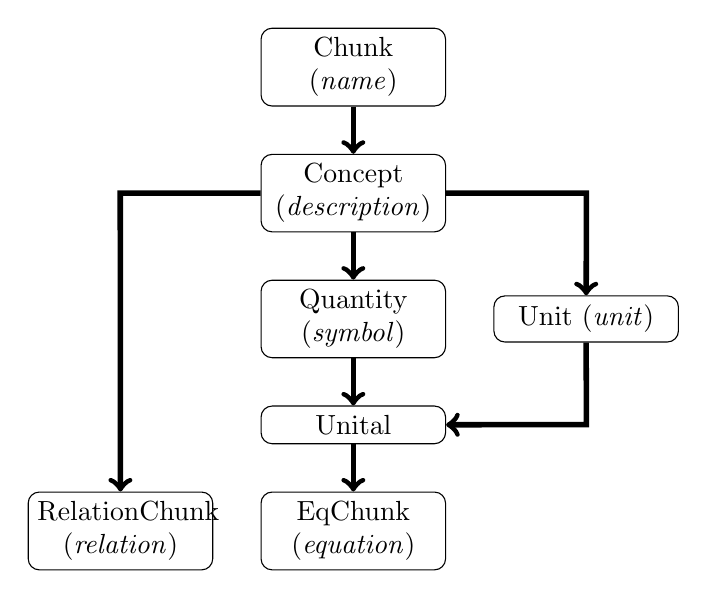
\begin{tikzpicture}[node distance=6mm]
  \tikzstyle{every node}=[draw,shape=rectangle, rounded corners,
    text width=6em, text centered];
  \node (ch)                     	{Chunk (\emph{name})};
  \node (co) [below = of ch]       {Concept (\emph{description})};
  \node (qu) [below = of co]  		{Quantity (\emph{symbol})};
  \node (u ) [right = of qu] 		{Unit (\emph{unit})};
  \node (uc) [below = of qu] 		{Unital};
  \node (eq) [below = of uc]	{EqChunk (\emph{equation})};
  \node (rc) [left = of eq]	{RelationChunk (\emph{relation})};

  \draw [->, line width=2pt] (ch) -- (co);
  \draw [->, line width=2pt] (co.west) -- (-2.96,-1.6) -- (rc); 
		%No idea how to do this
  \draw [->, line width=2pt] (co) -- (qu);
  \draw [->, line width=2pt] (co.east) -- (2.96,-1.6) -- (u );
  \draw [->, line width=2pt] (qu) -- (uc);
  \draw [->, line width=2pt] (u .south) -- (2.96,-4.54) -- (uc);
  \draw [->, line width=2pt] (uc) -- (eq);
\end{tikzpicture}
\end{center}
\caption{Our current chunk design (parentheses indicate newly added knowledge)}
\label{fig:chunks}
\end{figure}

Each new chunk in the hierarchy adds to the knowledge encapsulated within it.
The most basic \textit{Chunk} represents a named piece of information. A
\textit{Concept} adds a description to the named information, and so on.

\textit{Unital} chunks are somewhat special as they do not add any new
information in and of themselves, they act as a combination of a
\textit{Quantity} (concept with a symbolic representation) and a \textit{Unit}.
They are quantities with units.

\textit{Equation} chunks continue to expand on \textit{Unital} chunks by
allowing us to capture equations for calculating quantities. In a similar vein
are \textit{Relation} chunks, which allow us to relate two pieces of knowledge to
each other.

Now that knowledge has been encapsulated it is time to do something with it.
This is where the recipes, mentioned earlier, come into play. Writing a recipe
requires using three of the previously mentioned eDSLs -- the expression,
expression layout, and document layout languages. I will go into more detail on
writing and using recipes in the next section.

Finally, the last piece of the implementation is the generator. The remaining
three representation languages are specific to the generator. The generator
interprets the recipes and creates intermediary representations of artifacts
using the representation languages, then pretty-prints the results.

\subsection{Using Drasil}

For this section I will touch on two case studies that I have used to motivate
the development of Drasil. The first is a simplified version of a Software
Requirements Specification (SRS) for a fuel pin in a nuclear
reactor~\cite{SmithAndKoothoor2016} and the second is a SRS for a solar water
heating tank.

Let's start by looking at a single term from the fuel pin SRS: $h_c$. This term
represents the convective heat transfer coefficient between the clad and
coolant. We can see the data definition for this term in Figure~\ref{fig:h_c}.

\begin{figure}
~\newline \noindent \begin{minipage}{\textwidth}
\begin{tabular}{p{\colAwidth} p{\colBwidth}}
\toprule \textbf{Number} & \textbf{DD2 \label{hc}}
\\ \midrule 
Label & 
$h_{c}$
\\ \midrule
Units & $ML^0t^{-3}T^{-1}$\\ \midrule
SI Units & $\mathrm{\frac{kW}{m^{2o}C}}$\\ \midrule
Equation & $h_{c}$ =$
\frac{2k_{c}h_{b}}{2k_{c}+\tau_{c}h_{b}}$\\ \midrule
Description & $h_{c}$ is the convective heat transfer coefficient between clad
and coolant
\newline
$k_{c}$ is the
clad conductivity \newline
$h_{b}$ is the
initial coolant film conductance \newline
$\tau_{c}$ is the
clad thickness 
\newline
%NOTE: Equation taken from the code\\ \midrule  Sources & source code \\ \bottomrule 
\end{tabular} \end{minipage}\\ 
\caption{Data definition for $h_c$ from the fuel pin SRS}
\label{fig:h_c}
\end{figure}

From the data definition, we can glean interesting knowledge. First off there is
the name of the concept, its description, the symbol representing it, its SI
units, and its defining equation. All of this information can be encapsulated
into an EqChunk with ease as shown in Figure~\ref{fig:h_c_chunk}. Note that the
units for $h_c$ are defined in a piece of common knowledge known as
\verb|heat_transfer|.

\begin{figure}
\begin{lstlisting}[frame=single, showstringspaces=false, basicstyle=\small]
h_c_eq :: Expr
h_c_eq = 2*(C k_c)*(C h_b) /
  (2*(C k_c) + (C tau_c)*(C h_b))

h_c :: EqChunk
h_c = fromEqn "h_c" 
 "convective heat transfer coefficient
    between clad and coolant"
 (sub h c) heat_transfer h_c_eq
\end{lstlisting}
\caption{The $h_c$ chunk in Drasil}
\label{fig:h_c_chunk}
\end{figure}

The SI Units are a great example of common knowledge. The SI Unit library
contains all seven base SI units and several different derived units (for
example degrees Celsius, which are derived from Kelvin). The seven fundamental
base SI units implemented in Drasil can be seen in Figure~\ref{fig:SI}.

\begin{figure}
\begin{lstlisting}[frame=single, showstringspaces=false, basicstyle=\small, linewidth=13cm]
metre, second, kelvin, mole, kilogram, ampere, candela :: FundUnit
metre    = fund "Metre"    "length (metre)"               "m"
second   = fund "Second"   "time (second)"                "s"
kelvin   = fund "Kelvin"   "temperature (kelvin)"         "K"
mole     = fund "Mole"     "amount of substance (mole)"   "mol"
kilogram = fund "Kilogram" "mass (kilogram)"              "kg"
ampere   = fund "Ampere"   "electric current (ampere)"    "A"
candela  = fund "Candela"  "luminous intensity (candela)" "cd"
\end{lstlisting}
\caption{The seven fundamental SI Units in Drasil}
\label{fig:SI}
\end{figure}

From the captured knowledge and common knowledge, it is now possible to start
putting together a document using recipes. A small portion of the recipe for the
simplified fuel pin SRS can be seen in Figure~\ref{fig:recipe}. Currently the
recipes are fairly clunky and rely heavily on Haskell, but in the future this
will be improved. However, even with the current recipes we can see that the
output from the generator (Figure~\ref{fig:out}) is exactly what we want. Note:
the output I am showing is from the HTML version being generated, the TeX
version looks (almost) identical to the original SRS.

\begin{figure}[tb]
\begin{lstlisting}[frame=single, 
  showstringspaces=false, basicstyle=\scriptsize]
srsBody = srs [h_g, h_c] "Spencer Smith" [s1,s2,s3]

s1 = Section (S "Table of Units") [intro, table]

table = Table 
 [S "Symbol", S "Description"] (mkTable
   [(\x -> Sy (x ^. unit)),
    (\x -> S (x ^. descr)) ] si_units)

intro = Paragraph (S "Throughout this ...")
\end{lstlisting}
\caption{A portion of our simplified SRS recipe}
\label{fig:recipe}
\end{figure}

\begin{figure}
\centering
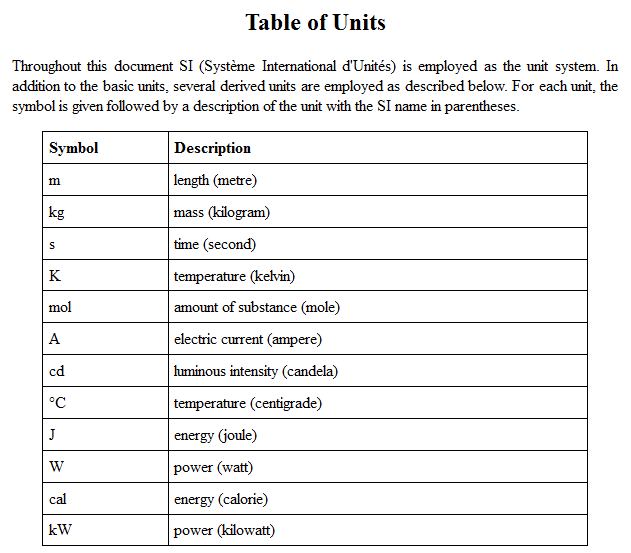
\includegraphics[scale=0.6]{HTML_out.png}
\caption{Section 1 of the generated SRS (HTML version)}
\label{fig:out}
\end{figure}

Already several advantages of using Drasil and a knowledge based approach are
obvious. First off, there are no inconsistencies in the knowledge both within
and across artifacts. Manually copying knowledge is no longer necessary, and we
can easily trace where a piece of knowledge came from. Should anything need
updating, the updates will automatically propagate throughout the artifacts when
the generator is run. We also have completely reusable knowledge (for example:
the SI Units) and the use of recipes supports design for change. As long as
knowledge is captured properly, it is as simple as changing a configuration file
to change the software.

One advantage that may seem like a disadvantage (but is not) is that of
pervasive bugs. Thanks to the full traceability and reuse of knowledge, a single
bug will be reproduced anywhere that piece of knowledge is necessary. This
improves the odds of finding it and makes it simple to fix. A single change
should update all of the artifacts and remove the bug.

There are a few disadvantages to using the knowledge based approach with Drasil.
The most obvious is the inability to include local hacks. Any human-modified
generated file will lose its modifications the next time the generator is run.

%Drasil also forces a sort of all-or-nothing aproach which removes meaningful
%iteration. The implementation must be done right the first time (or very close
%to it), requiring more development time. Also, the longer a project's lifecycle,
%the more involved the process of adding or modifying existing knowledge can
%become.

Finally, creating common-knowledge libraries is fairly difficult as it requires
a domain expert to be involved.

\section{Work Plan and Next Steps}

A full schedule of my work plan can be found in Table~\ref{table:sum_schedule}.
There are still many features I would like to add to Drasil as well as
improvements to the overall implementation. Currently anticipated additions and
changes (in no particular order) are as follows:

\begin{itemize}
\item Encapsulate more types of information in chunks. 
	Some of the next additions should be physical constraints and reasonable values.
\item Use constraints to generate test cases.
\item Implement much larger examples.
\item Generate code in more languages. Specifically MATLAB is the next planned output 
		language implementation.
\item Generate more artifact types. As it stands, the current recipes only create 
		requirements documents or code. New recipes should be included to cover design 
		documents, test cases, build instructions, user manuals, and more.
\item Generate different document views. This is partially implemented in the requirements 
		document recipe by allowing simplified or verbose data descriptions. The ability to 
		simplify parts of the document that are unnecessary for a target audience should be 
		expanded.
\item Create an external syntax for Drasil.
\end{itemize}

Over the summer (2016), three undergraduate students will be working on
translating existing implementations of large examples into Drasil
implementations. It is my hope that this experiment will provide insight on
any lacking features of Drasil, as well as how well the new approach works. A
second PhD student will also be joining the project over the summer. His first
task will involve implementing a large example and helping to expand Drasil.

\begin{table}
\caption{A detailed work schedule for the next twenty-eight months}
\begin{tabular}{|l|p{0.85\textwidth}|}
\hline
      Summer 2016 & Summer student experiment.
            Implement multiple (3-4) large examples using Drasil, updating the
              framework as new needs for features arise.
               
	Write up results of experiment as a paper and submit to SEHPCCSE'16.
				\\ \hline
      Fall 2016 & Overhaul the Drasil back-end to solidify necessary features
                      and re-design parts of the implementation.
                      
                      Finish PhD course requirements. 
                      
                      Meet with Ernie from OPG. 

\\ \hline
      Winter 2016 & Implement external syntax for Drasil. 

		Write a paper for ICSR (International Conference on Software Reuse).
      
      Write a journal paper for Automated Software Engineering.
\\ \hline
      Spring 2017 & Re-evaluate current Drasil implementation for usability. 
        Work on making it as user-friendly as possible. 

		Submit a paper to Onward!
		
		Submit a paper to ASE (International Conference on Automated Software Engineering)
        
      Meet with committee. 
\\ \hline
      Summer 2017 & Write a paper.
      
      Attempt to get summer students for second round of 
        experimentation.
        
        Write a journal paper detailing results.
\\ \hline
      Fall 2017 & Meet with Ernie from OPG. 
      
								 Update Drasil and perform a final evaluation. 
								 
\\ \hline
      Winter 2017 & Begin writing up full PhD Thesis.
\\ \hline
      Spring 2018 & Complete first draft of thesis and send to supervisors for 
        comments. Complete first round of edits.
\\ \hline
      Summer 2018 & Complete final thesis draft before defense. Make any
      necessary revisions to the thesis and submit it.
\\ \hline
\end{tabular}
\label{table:sum_schedule}
\end{table}


\newpage
\bibliography{drasil}
\newpage
%\appendix
%\section{Appendix}
%\label{app}
%\begin{table}[htp!]
%\caption{A detailed work schedule for the next twenty-eight months}
%\begin{tabular}{|l|p{0.85\textwidth}|}
%\hline
%      Summer 2016 & Summer student experiment.
%            Implement multiple (3-4) large examples using Drasil, updating the
%              framework as new needs for features arise.\\ \hline
%      June/July 2016 & Implement more artifact types in Drasil
%\\ \hline
%      August 2016 & Submit results of summer experimentation to SEHPCCSE'16
%\\ \hline
%      September 2016 & Overhaul the Drasil back-end to solidify necessary features
%                      and re-design parts of the implementation.
%\\ \hline
%      September 2016 & Begin the last course for my PhD requirements.
%\\ \hline
%      October 2016 & Meet with Ernie from OPG.
%\\ \hline
%      October 2016 & Begin implementation of more knowledge capture.
%\\ \hline
%      November 13, 2016 & (Hopefully) Present work at SEHPCCSE'16.
%\\ \hline
%      December 2016 & Finish coursework.
%\\ \hline
%      December 2016 & Write a paper.
%\\ \hline
%      January 2017 & Begin implementation of auto-generated test cases.
%\\ \hline
%      January 2017 & Begin work on external syntax.
%\\ \hline
%      February 2017 & Write a paper to submit to a journal.
%\\ \hline
%      March 2017 & Re-evaluate current Drasil implementation for usability. 
%        Work on making it as user-friendly as possible
%\\ \hline
%      April 2017 & Find and collect more large-scale examples to be implemented 
%        and begin implementation of one.
%\\ \hline
%      April 2017 & Meet with my committee.
%\\ \hline
%      May 2017 & Write a paper.
%\\ \hline
%      Summer 2017 & Attempt to get summer students for second round of 
%        experimentation. Complete implementation of multiple large-scale 
%        examples.
%\\ \hline
%      August 2017 & Write a paper to submit to a journal detailing the results.
%\\ \hline
%      September 2017 & Meet with Ernie from OPG.
%\\ \hline
%      Sept - Nov 2017 & Update Drasil and perform a final evaluation.
%\\ \hline
%      Dec 2017 & Begin writing up full PhD Thesis.
%\\ \hline
%      February 2018 & Complete first draft of thesis and send to supervisors for 
%        comments.
%\\ \hline
%      March 2018 & Begin editing thesis.
%\\ \hline
%      May 2018 & Complete final thesis draft before defense.
%\\ \hline
%      June 21, 2018 & Defend thesis.
%\\ \hline
%      July-August 2018 & Make any necessary revisions to the thesis, 
%        if major: defend again;
%        if minor: submit the finished copy.
%\\ \hline
%\end{tabular}
%\label{table:schedule}
%\end{table}
\end{document}




